% Preamble
\documentclass[12pt, a4paper]{report}

% Packages
\usepackage{titlesec,graphicx,tabularx,amsmath,indentfirst,multirow,nicefrac}
\usepackage[T2A] {fontenc}
\usepackage[russian]{babel}
\usepackage[utf8x] {inputenc}
\usepackage[top=2cm, bottom=2cm, left=1.5cm, right=1cm]{geometry}

\titleformat{\section}
{\Large\bfseries} % format
{}                % label
{0pt}             % sep
{\Large}          % before-code

\begin{document}
    \begin{footnotesize}
        \textit{\mbox{Федеральное государственное бюджетное образовательное учреджение высшего профессионального образования}}\\
    \end{footnotesize}

    \begin{tabular}{c c}
        \multirow{4}{*}{
\includegraphics[scale = 0.03]{mgtu.png}}
        & \\
        & \footnotesize\textit{\textbf{\guillemotleftМосковский государственный технический университет имени Н.Э. Баумана\guillemotright}}\\
        & \\
        & \textit{\textbf{(МГТУ им. Н.Э. Баумана)}}\\
        & \\
        & \\
        & \\
        \hline\\
    \end{tabular}

    ФАКУЛЬТЕТ \guillemotleftИнформатика и системы управления\guillemotright\\

    КАФЕДРА \guillemotleft Компьютерные системы и сети\guillemotright\\

    \vfill

    \begin{center}

        \textbf{Отчет}\\
        \bigskip
        \textbf{по домашнему заданию №3}\\
        \bigskip
        \textbf{Дисциплина: Электротехника}\\
        \bigskip
        \textbf{Название лабораторной работы:\\ Анализ переходных процессов электрической цепи.}\\
        \bigskip\bigskip
        \textbf{Вариант 19.}\\

        \vfill

        \begin{tabularx}{\textwidth}{X c r}
            Студент гр. ИУ6-35 & $\underset{\text{(Подпись, дата)}}{\makebox[2.0in]{\hrulefill}}$ & Т.Ш. Магомедов\\
            & & \\
            Преподаватель & $\underset{\text{(Подпись, дата)}}{\makebox[2.0in]{\hrulefill}}$ & С.Р. Иванов\\
        \end{tabularx}
        \bigskip\bigskip\bigskip\bigskip\\
        Москва, 2017
    \end{center}
    \thispagestyle{empty} % убрать номер страницы

    \newpage

    \section{\textbf{Задание}}
    \begin{flushleft}
        1. Для приведенного на чертеже принципиальной электрической схемы анализируемой цепи
        составить операторное представление выходного напряжения.\\
        2. Используя обратное преобразование Лапласа перейти к описанию выходного напряжения
        во временной области.\\
        3. Построить временные диаграммы переходного процесса, используя полученные формулы
        для него.\\
        4. Получить временные диаграммы для переходного процесса на выходе схемы с помощью
        пакета \guillemotleft Multisim\guillemotright.\\
        5. Сравнить полученные результаты между собой и сделатьзаключение о характере
        поведения анализируемой цепи.\\
    \end{flushleft}
    \bigskip\bigskip
    \section{\textbf{Схема цепи}}
    \begin{center}
        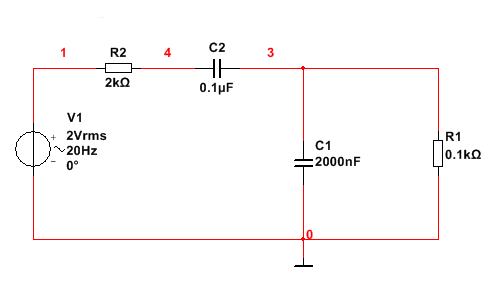
\includegraphics[scale = 3]{photo.png}\\
    \end{center}
    \textbf{Начальные условия:}
    \begin{itemize}
        $U_\text{вxm} = 2 \text{ B}$\\
        $F = 20 \text{ кГц}$\\
        $R_1 = 0,1 \text{ кОм}$\\
        $R_2 = 2 \text{ кОМ}$\\
        $C_1 = 2000 \text{ нФ}$\\
        $C_2 = 0,1 \text{ мкФ}$\\
        $U_{c}(0) = 2 \text{ В}$\\
        $U_\text{вых} = U_{R_1}$\\
    \end{itemize}
    \[ Z_{C_1} = \frac{1}{pC_1}; \>\>\>\>\>\>\>\> Z_{C_2} = \frac{1}{pC_2} \]

    \newpage

    \begin{center}
        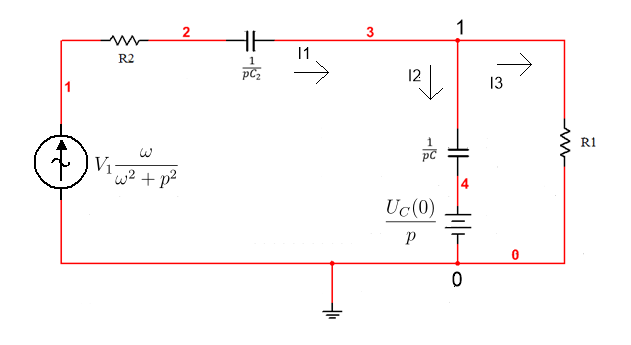
\includegraphics[scale = 0.8]{photo1.png}\\
        Представление расчетной схемы как опреаторный схемы замещения.\\
        \bigskip\bigskip\bigskip
        По первому закону Кирхгофа
    \end{center}
    \[ I_1 - I_2 - I_3 = 0 \]
    \[ I_1 = \frac{\varphi_0 - \varphi_1 + \frac{U_{m}\omega}{p^2 + \omega^2} } {R_2 + Z_{C_2}} \]
    \[ I_2 = \frac{ \varphi_1 - \varphi_0 - \frac{U_{C}(0)}{p} } {Z_{C_1}} \]
    \[ I_3 = \frac{\varphi_1 - \varphi_0}{R_1} \]\\
    \[ \frac{\varphi_0 - \varphi_1 + \frac{U_{m}\omega}{p^2 + \omega^2}}{R_2 + Z_{C_2}} - \frac{\varphi_1 - \varphi_0 - \frac{U_{C}(0)}p}{Z_{C_1}} - \frac{\varphi_1 - \varphi_0}{R_1} = 0 \]\\
    \[ \frac{Z_{C_1}R_1 \left( \frac{U_{m}\omega}{p^2 + \omega^2} - \varphi_1 \right) - \left( \varphi_1 - \frac{U_{C}(0)}{p} \right) \left( R_2 + Z_{C_2} \right)R_1 - \varphi_{1}\left( R_2 + Z_{C_2} \right)Z_{C_1}} {\left( R_2 + Z_{C_2} \right)Z_{C_1}R_1} = 0\]\\
    \[ \frac{\left( \frac{U_{m}\omega}{p^2 + \omega^2}Z_{C_1}R_1 + \frac{U_{C}(0)}{p}R_{1}R_2 + \frac{U_{C}(0)}{p}Z_{C_2}R_1  \right) - \varphi_{1}\left( Z_{C_1}R_1 + R_{1}R_2 + Z_{C_2}R_1 + Z_{C_1}Z_{C_2} + Z_{C_1}R_2 \right) } {\left( R_2 + Z_{C_2} \right)Z_{C_1}R_1} = 0 \]\\
    \[ \varphi_1 = U(p) = \frac{ \frac{U_{m}}{p^2 + \omega^2} \frac{1}{pC_1}R_1 + \frac{U_{C}(0)}{p}R_{1}R_2 + \frac{U_{C}(0)}{p}\frac{1}{pC_2}R_1 } {\frac{1}{pC_1}R_1 + R_{1}R_2 + \frac{1}{pC_2}R_1 + \frac{1}{pC_1}R_2 + \frac{1}{pC_1}\frac{1}{pC_2} } \]\\
    \[ U(p) = \frac{ \left( U_{m}\omega R_{1}pC_2 + U_{C}(0)pR_{1}R_{2}C_{1}C_{2}(p^2 + \omega^2) + U_{C}(0)R_{1}C_{1}(p^2 + \omega^2) \right)pC_{1}C_{2} } { ( pC_{2}R_{1} + pC_{1}pC_{2}R_{1}R_{2} + pC_{1}R_{1} + pC_{2}R_{2} + 1)(p^2 + \omega^2)pC_{1}C_{2} } \]

    \newpage

    Тогда операторное представление выходного напряжения будет выглядеть следующим образом
    \[ U(p) = R_{1}\frac{U_\text{вxm}C_{2}\omega p + U_{c}(C_1 + pC_{1}C_{2}R_2)(p^2 + \omega^2)} {{(p^2 + \omega^2)(1 + pC_{2}R_{2} + pC_{1}R_{1} + pC_{2}R_{1} + p^2C_{1}C_{2}R_{1}R_{2})}} \]
    Решим характеристическое уравнение
    \[ (p^2 + \omega^2)(1 + pC_{2}R_{2} + pC_{1}R_{1} + pC_{2}R_{1} + p^2C_{1}C_{2}R_{1}R_{2}) = 0 \]
    Корни
    \[ p_{1,2} = \pm j\omega \]
    \[ p^2(C_{1}C_{2}R_{1}R_{2}) + p(C_{2}R_1 + C_{1}R_1 + C_{2}R_2) + 1 = 0 \]\\
    \[ p_{3,4} = \frac{-(C_{2}R_1 + C_{1}R_1 + C_{2}R_2) \pm \sqrt{(C_{2}R_1 + C_{1}R_1 + C_{2}R_2)^2 - 4C_{1}C_{2}R_{1}R_{2}}} {2C_{1}C_{2}R_{1}R_{2}} \]\\
    \begin{equation*}
        \begin{cases}
            p_1 = 125663,7j\\
            p_2 = - 125663,7j\\
            p_3 = - 6250\\
            p_4 = - 4000\\
        \end{cases}
    \end{equation*}
    \[ U_\text{вxm}(t) = \sum_{i = 1}^{4}\frac{F_{1}(p_i)} {F_{2}^\prime (p_i)}e^{p_{i}t} \]\\
    \[ F_{2}^\prime = (p^2 + \omega^2)(C_{2}R_{2} + C_{1}R_{1} + C_{2}R_{1} + 2pC_{1}C_{2}R_{1}R_{2}) + \]
    \[ + {1 + 2p(pC_{2}R_{2} + pC_{1}R_{1} + pC_{2}R_{1} + p^2C_{1}C_{2}R_{1}R_{2})} \]\\
    \[ F_{2}^\prime = (p^2 + 15791365497,7)( 0,00001 + 0,0002 + 0,0002 + 0,00000008p) +\]
    \[ + 2p(1 + 0,00001p + 0,0002p + 0,0002p + 0,00000004p^2)\]\\
    \[ F_1 = 100 \times (0,025p + 2 \times (2000 * 10^{-9} + p^2 \times 40 * 10^{-9}) (p^2 + 15791365497,7)) \]\\
    \[ F_{1}(p_3) = - 1598750,8 \]
    \[ F_{1}(p_4) = 1254536.4 \]\\
    \[ F_{2}^{\prime}(p_3) = - 1424738.5\]
    \[ F_{2}^{\prime}(p_4) = 1422662.9 \]

    \newpage

    \[ \frac{F_{1}(p_1)} {F_{2}^\prime (p_1)}e^{p_{1}t} = \frac{U_\text{вxm}C_{2}R_1\omega} {2(1 + C_{2}R_{2}j\omega + C_{1}R_{1}j\omega + C_{2}R_{1}j\omega - \omega^2C_{1}C_{2}R_{1}R_{2})}e^{j\omega t} \]\\
    \[ \frac{F_{1}(p_2)} {F_{2}^\prime (p_2)}e^{p_{2}t} = \frac{-U_\text{вxm}C_{2}R_1\omega} {-2(1 - C_{2}R_{2}j\omega - C_{1}R_{1}j\omega - C_{2}R_{1}j\omega - \omega^2C_{1}C_{2}R_{1}R_{2})}e^{-j\omega t} \]\\

    \[ \text{Обозначим} \textit{ D} = \frac{U_\text{вxm}C_{2}R_1\omega} {2((C_{2}R_{2}j\omega + C_{1}R_{1}j\omega + C_{2}R_{1}j\omega)^2 + (1 - \omega^2C_{1}C_{2}R_{1}R_{2})^2)} \]\\
    Для суммы первых двух слагаемых
    \[ D(e^{j\omega t}(-j(C_{2}R_{2}\omega + C_{1}R_{1}\omega + C_{2}R_{1}\omega)^2 + (1 - \omega^2C_{1}C_{2}R_{1}R_{2})^2) + \]
    \[ + e^{-j\omega t}(j(C_{2}R_{2}\omega + C_{1}R_{1}\omega + C_{2}R_{1}\omega)^2 + (1 - \omega^2C_{1}C_{2}R_{1}R_{2})^2)) = \]
    \[ = D\left( \frac{e^{j\omega t} + e^{-j\omega t}}{1} (1 - \omega^2C_{1}C_{2}R_{1}R_{2}) - \frac{e^{j\omega t} - e^{-j\omega t}}{1} j(C_{2}R_{2}\omega + C_{1}R_{1}\omega + C_{2}R_{1}\omega) \right) \]\\
    Домножаем и делим второе слагаемое на \textit{j} и выносим из общей части \nicefrac{1}{2}
    \[ D\left( \frac{e^{j\omega t} + e^{-j\omega t}}{2} (1 - \omega^2C_{1}C_{2}R_{1}R_{2}) - \frac{e^{j\omega t} + e^{-j\omega t}}{2j}(C_{2}R_{2}\omega + C_{1}R_{1}\omega + C_{2}R_{1}\omega) \right) = \]
    \[ D\left( \cos(\omega t)(1 - \omega^2C_{1}C_{2}R_{1}R_{2}) + \sin(\omega t)(C_{2}R_{2}\omega + C_{1}R_{1}\omega + C_{2}R_{1}\omega) \right) \]\\
    \[ \frac{U_\text{вxm}C_{2}R_1\omega} {2((C_{2}R_{2}j\omega + C_{1}R_{1}j\omega + C_{2}R_{1}j\omega)^2 + (1 - \omega^2C_{1}C_{2}R_{1}R_{2})^2)} \times \]
    \[ \times \left( \cos(\omega t)(1 - \omega^2C_{1}C_{2}R_{1}R_{2}) + \sin(\omega t)(C_{2}R_{2}\omega + C_{1}R_{1}\omega + C_{2}R_{1}\omega) \right) = \]
    \[ = \frac{2,5} {((51,5)^2 + (-630,7)^2)} \times \left( \cos(125663,7t)(-630,7) + \sin(125663,7t)(51.2) \right) = \]
    \[ = -0,004 \times \cos(125663,7t) + 0,0003 \times \sin(125663,7t) \]\\
    \[ U_\text{выхm}(t) = -0,004\cos(125663,7t) + 0,0003\sin(125663,7t) + 1,1e^{-6250t} + 0,9e^{-4000t} \]
    \[ \arctg\left( \frac{-0,004}{3} \right) = 0,00013 \]
    \[ U_\text{вых}(t) = 3\sin(125663,7t) + 0,00013^{\circ} + 1,1e^{-6250t} + 0,9e^{-4000t} \]

    \newpage

    \begin{center}
        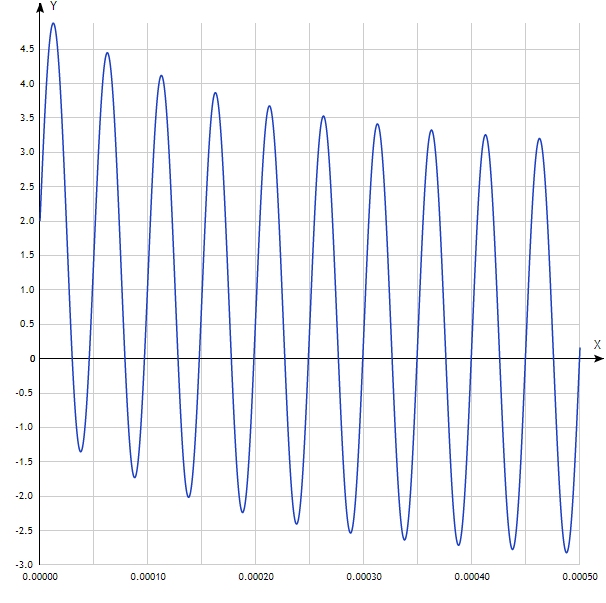
\includegraphics[scale = 0.9]{photo2.png}\\\bigskip
        Рис.3 - Построенный итоговый график\\\vfill
        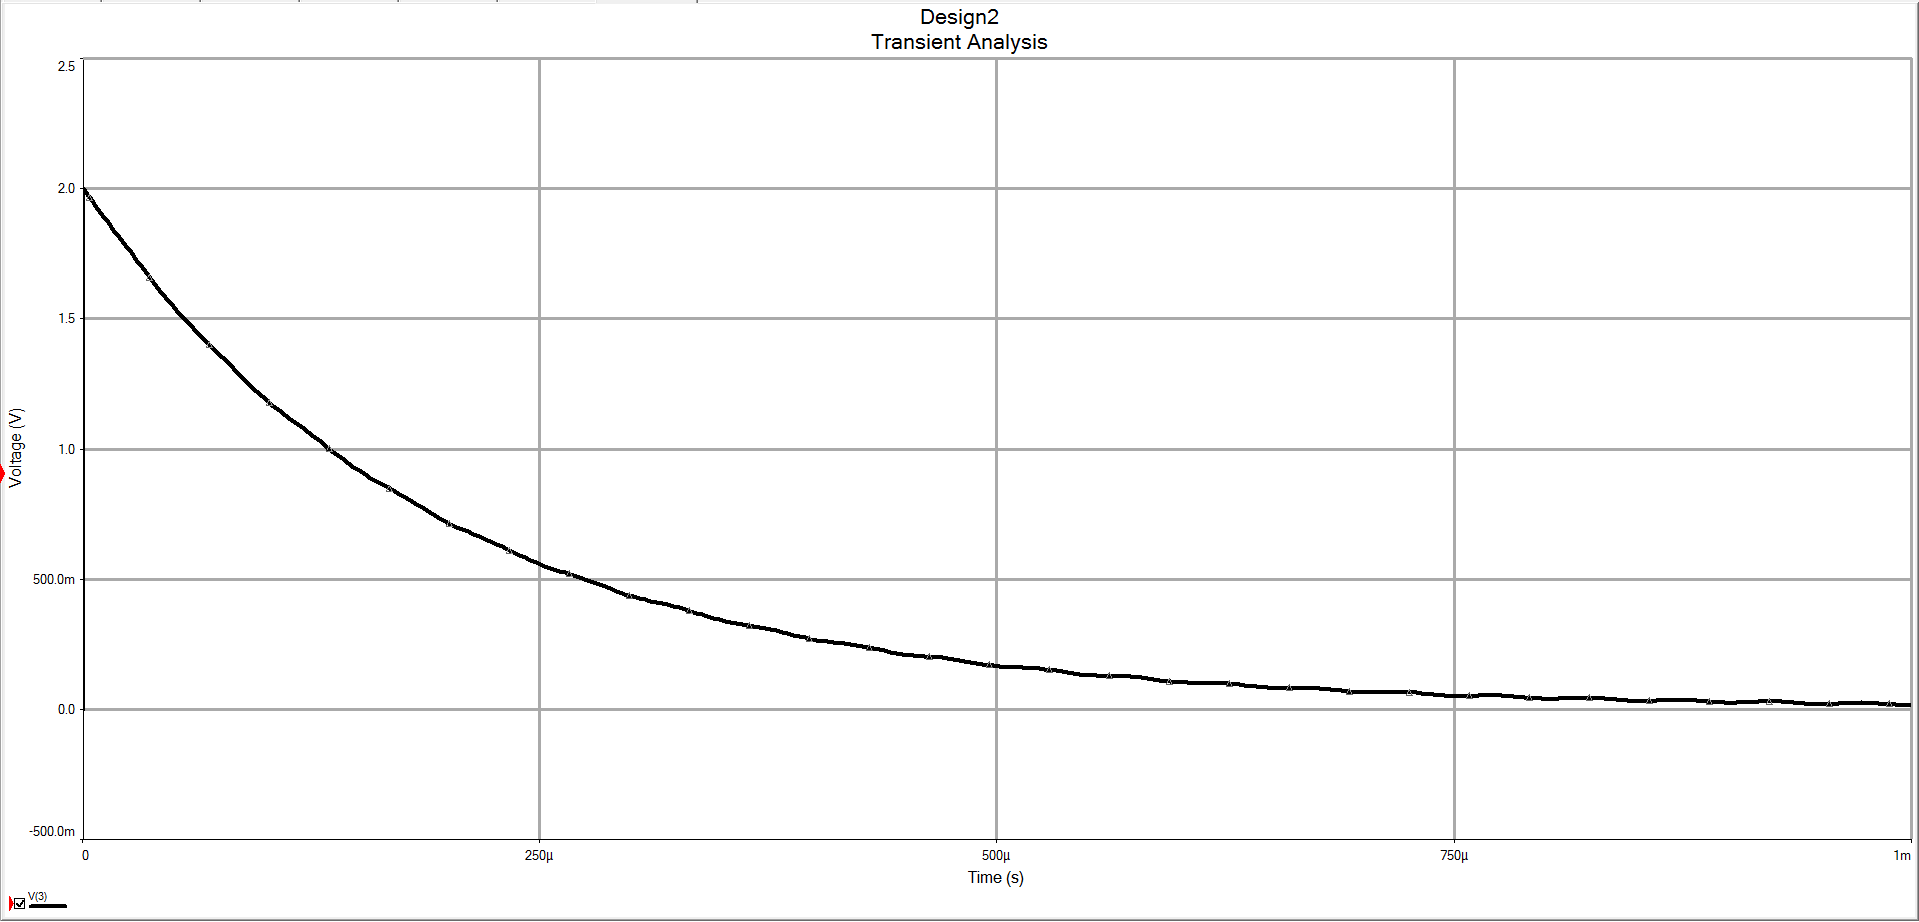
\includegraphics[scale = 0.3]{photo3.png}\\\bigskip
        Рис.4 - График начального условия
    \end{center}

    \newpage

    \begin{center}
        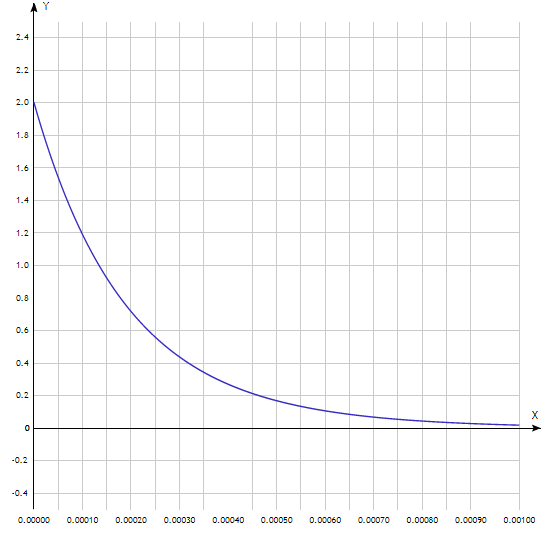
\includegraphics[scale = 1]{photo4.png}\\\bigskip
        Рис.5 - График экспоненты
    \end{center}
\end{document}